\documentclass[12pt]{scrartcl}

\usepackage{graphicx}
\usepackage{paralist}
\usepackage{amsfonts}
\usepackage{amsmath}
\usepackage{hhline}
\usepackage{booktabs}
\usepackage{multirow}
\usepackage{multicol}
\usepackage{makecell}


\oddsidemargin 0mm
\evensidemargin 0mm
\textwidth 160mm
\textheight 200mm
\renewcommand\baselinestretch{1.0}

\pagestyle {plain}
\pagenumbering{arabic}

\newcounter{stepnum}

\usepackage{color}


\title{Get it Done (v2.0)}
\subtitle{SFWRENG 2XB3 - Computing and Software - McMaster University}
\author{Group 14 - Immanuel Odisho, Ninos Yomo, Paul Heys, \\ Justin Zhou, Will Donaldson}
\date{3 April 2018}
\begin {document}

\newpage

\maketitle

The purpose of this document is to  povide a description of the classes/modules we have decided to use in our application, and explain why we have decomposed the application into these classes. We have included a UML class diagram showing a static representation of our application classes and the relationship between classes.

Also, for each class, a description of the interface (public entities) as well as a description of the syntax is provided.

\newpage

\section* {Revision Page}

\subsection*{Team Members and Roles}
$
\newline
$
\begin{tabular}{| l | l | l |}
\hline
\textbf{Team member} & \textbf{Student No.} & \textbf{Roles/Responsibilites} \\
\hline
Immanuel Odisho & 400074199 & \makecell{Design Specifications manager \\ Graph processing and GUI researcher } \\
\hline
Paul Heys & ---- & \makecell{Project Leader \\ Sorting Algorithm implementation researcher \\ Sorting algorithm implementer\\} \\
\hline
Ninos Yomo  & ------- &\makecell{ADT developer \\ class relation manager \\ Database researcher } \\
\hline
Justin Zhou & ------ & \makecell{log administrator \\ file manager \\ specifications contributer} \\
\hline
Will Donaldson & ----- & \makecell{Testing \\ Verification and Validation bookkeeper \\ Searching algorthm researcher and implementer} \\
\hline
\end{tabular}


\subsection*{Attestation and Consent:}

\textit{By virtue of submitting this document we electronically sign and date that the  work  being  submitted  by  all  the  individuals  in  the  group  is  their  ex-clusive work as a group and we consent to make available the application developed  through  [CS]  or  [SE]-2XB3  project,  the  reports,  presentations,and assignments (not including my name and student number) for futureteaching purposes.}

\newpage

\section* {Contribution Page}

\subsection*{Team Members, Roles and Contributions}
$
\newline
$
\begin{tabular}{| l | l | l |}
\hline
\textbf{Team member} & \textbf{Roles/Responsibilities} & \textbf{Contributions} \\
\hline
Immanuel Odisho & \textit{same as previous page} & \makecell{Design Specifications Document \\ Graph processing GUI, \\ Reviews interface (front end)} \\
\hline
Paul Heys & \textit{same as previous page} & \makecell{Sorting algorithm \\ Graph Processing (back end)} \\
\hline
Ninos Yomo  & \textit{same as previous page} &\makecell{ContractorADT, GUI splash screen, \\ main menu and search results display (front end) \\  } \\
\hline
Justin Zhou & \textit{same as previous page} & \makecell{Data Reader module \\ log administrator} \\
\hline
Will Donaldson & \textit{same as previous page}  & \makecell{Searching algorithm \\ verification and validation, \\ Debugging } \\
\hline
\end{tabular}

\subsection* {Executive Summary}

The goal of this project is to connect Washingtonians who need contracting work done to the people with the skills to do it. The consumer will be able to enter information about the type of work they want done and how they want it done. This information will be used to identify contractors who meet their needs using the license data of all contractors in the state of Washington. Users will be connected to contactors who specialize in those fields ranked by user given reviews. \footnote{This abstract was taken from $\textit{MileStone1\_Group14.docx}$}

\newpage 

\tableofcontents 

\newpage

\section {ContractorADT Module}

\subsection{Template Module}

Contractor

\subsection {Uses}

N/A

\subsection {Syntax}

\subsubsection {Exported Types}

Contractor = ?

\subsubsection {Exported Access Programs}

\begin{tabular}{| l | l | l | l |}
\hline
\textbf{Routine name} & \textbf{In} & \textbf{Out} & \textbf{Exceptions}\\
\hline
$Contractor$ & \makecell{$String$, $String$, $String$,$String$,$String$,\\ $String$,$String$,$String$,$String$,$\mathbb{Z}$}  & $Contractor$ & \\
\hline
$Contractor$ & $String$, $String$, $String$ & $Contractor$ & ~\\
\hline
isActive & ~ & $\mathbb{B}$ & ~\\
\hline
getLicenseNumber & ~ &  $\mathbb{Z}$ &
\\
\hline
getAddress & ~ & $String$ & \\
\hline
getContractorName & ~ & $String$ & \\
\hline 
getCity & ~ & $String$ & \\
\hline 
getState & ~ & $String$ & \\
\hline 
getSpecialty & ~ & $String$ & \\
\hline 
CompareTo & $Contractor$ & $\mathbb{Z}$ & \\
\hline 
avgReview & $Map$ & $String$ & \\
\hline 
\end{tabular}

\subsection {Semantics}

\subsubsection {State Variables}

businessName: $String$\\
licenseNumber: $String$\\
address: $String$\\
city: $String$\\
state: $String$\\
zip: $String$\\
number: $String$\\
specialty: $String$\\
contractorName: $String$\\
activeLicense: $\mathbb{Z}$

\subsubsection {State Invariant}

None

\subsubsection {Assumptions}

The constructor Contractor is called for each object instance before any other
access routine is called for that object.  The constructor cannot be called on
an existing object.

\subsubsection {Access Routine Semantics}

Contractor($Name,License,address,city,state,zip,number,specialty, contractorName, acLicense$):
\begin{itemize}
\item transition: $ businessName, licenseNumber, address, city, state, zip, \\ number, specialty, contractorName, activeLicense:= Name,License, address,city,\\ state,zip,number,specialty, contractorName,acLicense$
\item output: $out := \mathit{self}$
\item exception: None
\end{itemize}

\noindent contractor(city1,state1,specialty1):
\begin{itemize}
\item transition: $city, state, specialty := city1, state1, specialty1$
\item exception: None
\end{itemize}

\noindent isActive():
\begin{itemize}
\item output: $out := (activeLicense = 1) \Rightarrow True | False$
\end{itemize}

\noindent getLicenseNumber():
\begin{itemize}
\item output: $out := licenseNumber$
\end{itemize}


\noindent getAddress():
\begin{itemize}
\item output: $out := address$
\end{itemize}

\noindent getContractorName():
\begin{itemize}
\item output: $out := businessName$
\end{itemize}

\noindent getCity():
\begin{itemize}
\item output: $out := city$
\end{itemize}

\noindent getState():
\begin{itemize}
\item output: $out := state$
\end{itemize}

\noindent getSpecialty():
\begin{itemize}
\item output: $out := specialty$
\end{itemize} 

\noindent compareTo(that):
\begin{itemize}
\item output: $out := \neg (self.getActive() = that.getActive()) \Rightarrow ((self.getActive() = True) \Rightarrow 1 | False) $ 
\end{itemize} 

\noindent avgReview(map):
\begin{itemize}
\item output: $out := \neg (self.getActive() = that.getActive()) \Rightarrow ((self.getActive() = True) \Rightarrow 1 | False) $ 
\end{itemize} 


\newpage

\section {Search Module}

\subsection{Template Module}

Search

\subsection {Uses}

Contractor \\
DataReader \\
Reviews

\subsection {Syntax}

\subsubsection {Exported Types}

N/A

\subsubsection {Exported Access Programs}

\begin{tabular}{| l | l | l | l |}
\hline
\textbf{Routine name} & \textbf{In} & \textbf{Out} & \textbf{Exceptions}\\
\hline
search & seq of Contractor, Contractor, String & seq of Contractor & IOException\\
\hline
\end{tabular}

\subsection {Semantics}

\subsubsection {State Variables}

N/A

\subsubsection {State Invariant}

None

\subsubsection {Assumptions}

N/A

\subsubsection {Access Routine Semantics}

search(Contractors,Contractor,filename):
\begin{itemize}
\item output: out := $\{c : Contractor | c \in Contractors : \\ ((c.getCity() = Contractor.getCity()) \wedge (c.getState() = Contractor.getState()) \wedge (c.getSpecialty() = Contractor.getSpecialty()) | c.getSpecialty() = General) \Rightarrow c \}$
\item exception: None
\end{itemize}


\newpage

\section {Sort Module}

\subsection{Template Module}

Sort

\subsection {Uses}

Contractor \\
DataReader \\
Reviews 

\subsection {Syntax}

\subsubsection {Exported Types}

N/A

\subsubsection {Exported Access Programs}

\begin{tabular}{| l | l | l | l |}
\hline
\textbf{Routine name} & \textbf{In} & \textbf{Out} & \textbf{Exceptions}\\
\hline
sort & seq of Contractor &  & \\
\hline
isSorted & seq of Contractor & $\mathbb{B}$ & \\
\hline

\end{tabular}

\subsection {Semantics}

\subsubsection {State Variables}

N/A

\subsubsection {State Invariant}

None

\subsubsection {Assumptions}

N/A

\subsubsection {Access Routine Semantics}

isSorted(Contractors):
\begin{itemize}
\item output: out := $\forall (i : \mathbb{N} | i \in [0..|Contractors|-2] : (Contractors[i].compareTo(Contractors[i+1]) <= 0)$
\item exception: None
\end{itemize}

sort(Contractors):
\begin{itemize}
\item output: out := $Contractor^n$ such that $\forall(c : Contractor | c \in Contractors : \exists(b : Contractor | b \in B : b.compareTo(c) = 0 \wedge count(c,Contractors) = count(b,B))) \wedge isSorted(B)$
\item exception: None
\end{itemize}

\subsubsection {Local Funtions}

$count(a,A) : Contractor \times Contractor^n$ \\
$count(a,A) \equiv +(i : \mathbb{N} | i \in [0..|A|-1] \wedge A[i].compareTo(a) = 0 : 1)$ \\

\newpage


\section {Data Reader Module}

\subsection{Template Module}

DataReader

\subsection {Uses}

Contractor


\subsection {Syntax}

\subsubsection {Exported Types}

N/A

\subsubsection {Exported Access Programs}

\begin{tabular}{| l | l | l | l |}
\hline
\textbf{Routine name} & \textbf{In} & \textbf{Out} & \textbf{Exceptions}\\
\hline
readContractors & & seq of Contractor  & \\
\hline
\end{tabular}

\subsection {Semantics}


\subsection {Environment Variables}

dataset: two dimensional sequence of text characters

\subsubsection {State Variables}

None

\subsubsection {State Invariant}

None

\subsubsection {Assumptions}

None

\subsubsection {Access Routine Semantics}

readContractors():
\begin{itemize}
\item transition:  When this method is called it will read through the \textit{FullData.txt} data set and then create a list of Contractor objects and return a list of all the objects made.
\item output: out := seq of Contractor
\item exception: None
\end{itemize}


\newpage

\section {Reviews Module}

\subsection{Template Module}

Reviews

\subsection {Uses}

None

\subsection {Syntax}

\subsubsection {Exported Types}

N/A

\subsubsection {Exported Access Programs}

\begin{tabular}{| l | l | l | l |}
\hline
\textbf{Routine name} & \textbf{In} & \textbf{Out} & \textbf{Exceptions}\\
\hline
initMapFromFile & s: String &  Map & \\
\hline
avgOfContractor & licenseNumber:String, Map & string &\\
\hline 
addReview & Map, licenseNumber:String, s: String & & \\
\hline
writeMapToFile & Map, filename:String & & \\
\hline
\end{tabular}

\subsection {Semantics}


\subsubsection {State Variables}

None

\subsubsection {State Invariant}

None

\subsubsection {Assumptions}

None

\subsubsection {Access Routine Semantics}

initMapFromFile(s):
\begin{itemize}
\item transition:  This method is called it will load the \textit{Reviews.txt} database into the program and return a map object of all the Contractors' reviews.
\item output: out := Map object with contractor license number as key and corresponding contractor's reviews as value.
\item exception: None
\end{itemize}


avgOfContractor(licenseNumber,Map):
\begin{itemize}
\item output: out := average review of contractor with corresponding license number in the Map object.
\item exception: None
\end{itemize}

addReview(Map, licenseNumber, s):
\begin{itemize}
\item transition: add the review as a value in Map with the corresponding license number as a key.
\item exception: None
\end{itemize}

writeMapToFile(Map,filename):
\begin{itemize}
\item transition: write the information in a file with the name of filename only when the program is shutdown.
\item exception: None
\end{itemize}


\newpage

\section {GUI Package}

\subsection{Package Module}

GUI

\subsection {Uses}

Contractor \\
Search \\
Sort \\
DataReader \\
Reviews \\

\subsection {Syntax}

\subsubsection {Exported Types}

N/A

\subsection {Semantics}

\subsection{Environment variables}

win: two dimensional and interactive sequence of coloured pixels \footnote{this definition was taken from SFWRENG 2AA4 2018 Assignment 2 specifications.}

\subsubsection {State Variables}

None

\subsubsection {State Invariant}

None

\subsubsection {Assumptions}

None

\subsubsection {Implementation}

Using the specifications from the other modules, implement the specifications with a graphical user interface in the win environment variable.

\newpage 

\section {UML between public classes}


\begin{center}
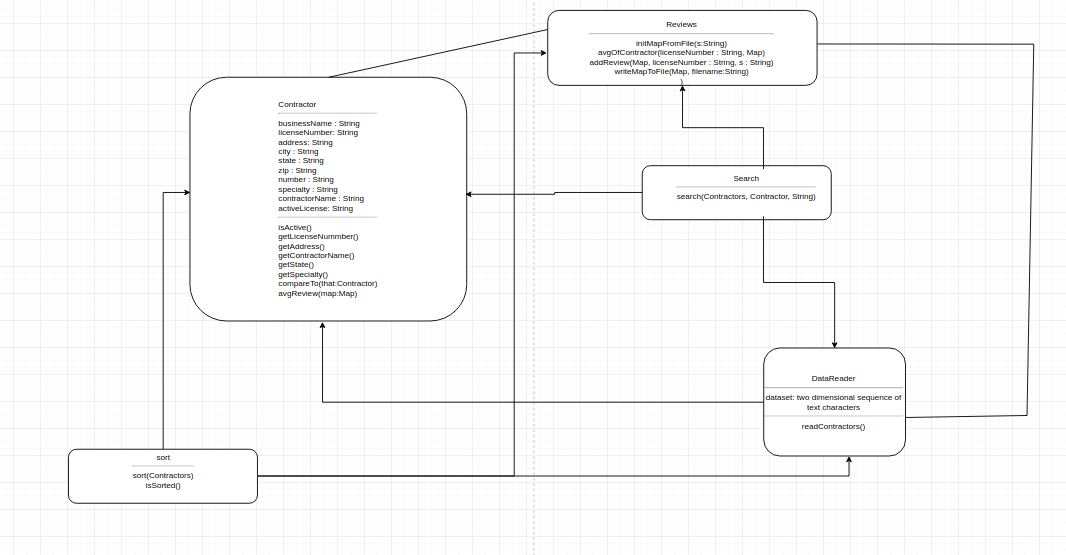
\includegraphics[angle = 270, scale = 0.70]{uml.png}
\end{center}


\end {document}\grid
